\documentclass[10pt]{article}
\usepackage[final]{pdfpages}
\usepackage{cleveref}
\usepackage{xparse}
\usepackage[hidelinks]{hyperref}
\usepackage{geometry}
\usepackage{amsmath}
\usepackage{graphicx}
\usepackage{caption}
\usepackage{subcaption}
\usepackage[section]{placeins}
\usepackage{listings}
\usepackage{verbatim}
\usepackage[dcucite,abbr]{harvard}
\usepackage{sectsty}
\usepackage{html}
\usepackage{url}
\usepackage[section]{placeins}

\usepackage{helvet}
\renewcommand{\familydefault}{\sfdefault}
\geometry{
 %body={6.5in, 8.5in},
 left=2.5cm,
 right=2cm,
 top=2cm,
 bottom=2cm
}

\linespread{1.213}
\makeindex
\begin{document}
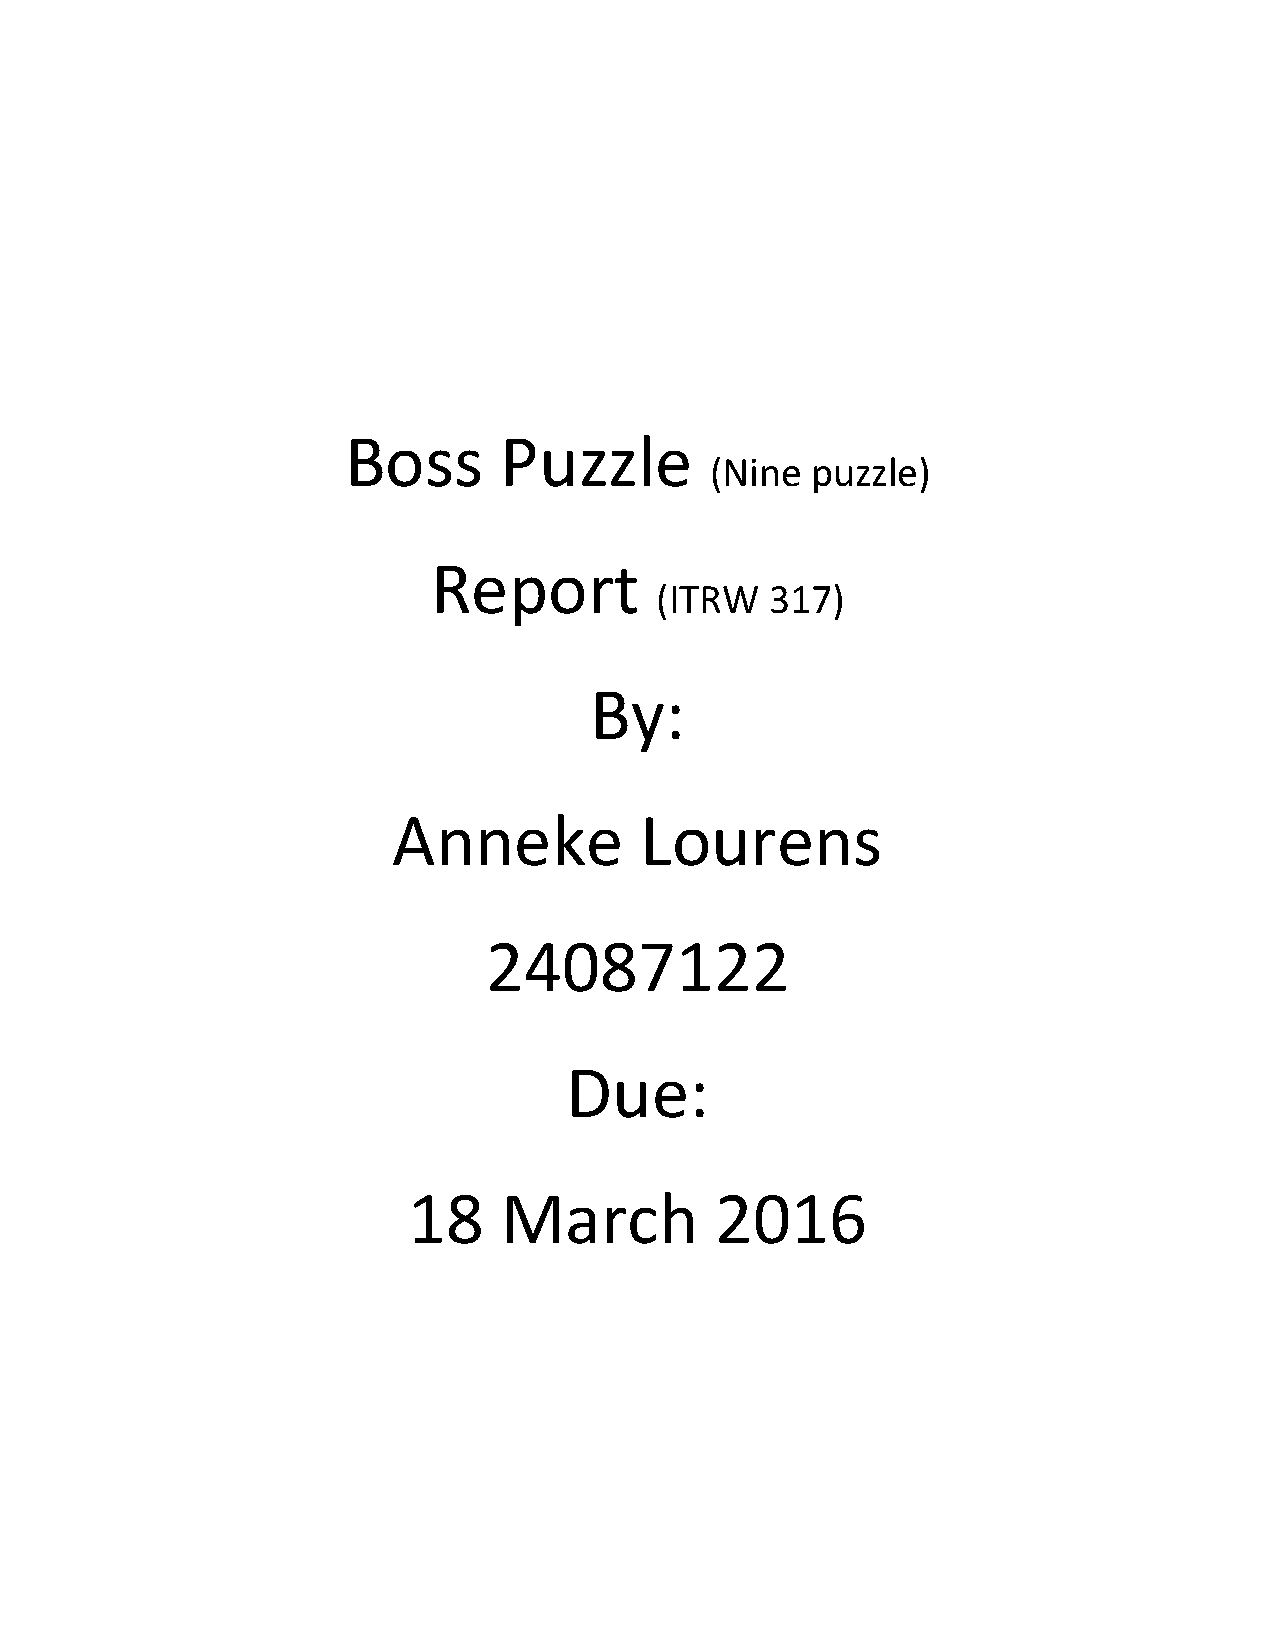
\includepdf{./BossPuzzle.pdf}
\tableofcontents
\pagebreak
\section{Introduction}
\subsection{Background}
The nine puzzle is a $3 \times 3$ board with eight tiles also called cells, and the ninth one is blank space. The blank space is always in the lower right corner of the puzzle. The objective of the nine puzzle is to slide the tiles/cells into the space to make a picture complete or arrange the tiles in numerical order. The nine puzzle is the only puzzle that can be completely solved. If we look at the nine puzzle, there are 9! permutations that the board can be solved\cite{reinefeld1993complete}. There are $9!/2 = 181 440$ possible ways to solve the nine puzzle. The problem requires an average of 22 moves to complete the puzzle \cite{reinefeld1993complete}.  The nine puzzle cannot be solved if the numbers one to seven is arranged in order from left to right, top to bottom with the seventh and eight number that has been switched. 
We want to optimize the moves so that the puzzle can be solved in the fewest moves. The $n$ puzzle is considered an NP-Hard problem when the minimum amount of moves need to be answered.
\section{Literature Study}
\subsection{History}
Sam Loyd, the impish puzzle maker, introduced the 15-puzzle to the United States, Britain, and Europe in the 1870's.\cite{archer1999modern}.  The original fifteen puzzle had numbers from 1 - 15 on the tiles.  If one would have bought the 15 puzzle back then the numbers from 1 to 13 was arranged in the right order from left to right, top to bottom with the blank space in the lower right corner, and the 14 and 15 have been reversed. Loyd drove the world crazy with the puzzle, and he offered \$1 000 to the first person that could solve the problem. The 15 puzzle was impossible to solve if the numbers 14 and 15 has been switched. The 15 puzzle cannot be solved with the blank space in the lower right corner.  It is only possible to address the problem if there are an even number of moves, so the resulting permutation is even \cite{archer1999modern}.
\\
\\The puzzle then becomes in many sizes.  Like the nine puzzle that is the smallest and there exists a 24 puzzle as well.
\section{User Guide}
\subsection{How to make a .csv file}
Open the file named "waarde\_puzzle.csv" in your favorite text editor e.g. Notepad$++$, Notepad, Vim, Nano.
If you want to change the order of the numbers, just remember that there must only be a "," the numbers in between the numbers. The numbers that are used is 1 to 8 and a lowercase "b" that will represent the blank space Figure~\ref{csv}.
\\
\\Figure~\ref{waardes} is an example of what the .csv file looks like in Notepad$++$ or Notepad. \\The first row in the file is the initial puzzle that the player must solve according to the solved puzzle. The second row in the file is the solved puzzle. If the player has saved the puzzle to continue at a later stage, then there will be a third row in the .csv file that shows the moves that the player has made already.
\begin{figure}
\centering
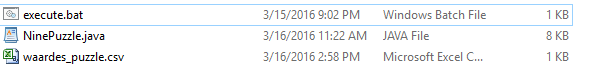
\includegraphics[scale=0.7]{./Prente/csv.png}
\caption{This is the files that one get which will run the nine puzzle}
\label{csv}
\end{figure}
\begin{figure}
\centering
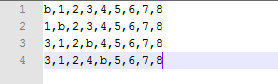
\includegraphics[scale=1]{./Prente/waardes.png}
\caption{How the data looks in the .csv file. This data will be used in the nine puzzle.}
\label{waardes}
\end{figure}
\FloatBarrier
\subsection{How to begin the Nine-puzzle}
Step 1:
\\If you have your own .csv file - right click on the execute.bat file and open it in Notepad$++$ or Notepad Figure~\ref{csv}.
Change the file name of the .csv file to your own .csv file's name. Save the execute.bat file and exit it.
\\Double-click on the execute.bat file to run the program Figure~\ref{begincmd}. 
\\
\\Step 2:
\begin{figure*}
  \centering
  \begin{subfigure}{0.5\textwidth}
    \centering
    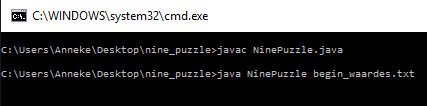
\includegraphics[scale=0.8]{./Prente/begincmd.png}
    \caption{If you have run the execute.bat file this lines will show in the CMD }
    \label{begincmd}
  \end{subfigure}%
~ 
  \begin{subfigure}{0.5\textwidth}
    \centering
    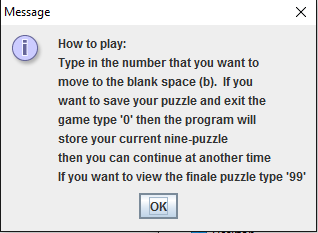
\includegraphics[scale=0.8]{./Prente/MessageBegin.png}
    \caption{The how to play message after you have run the execute.bat file}
    \label{MessageBegin}
  \end{subfigure}
  \caption{The beginning of the program\label{1}}
  \end{figure*}
\\If the program has run correctly then you will get a message telling you how to play the nine puzzle. Figure~\ref{MessageBegin} shows the message dialog to inform the player on the rules of the nine-puzzle game.
\\
\\Step 3: 
\\Enter a "y" for you are a new player or "n" for you are not a new player. Figure~\ref{prent1} shows how the program asks if you are a new player of not.
\begin{figure}
\centering
 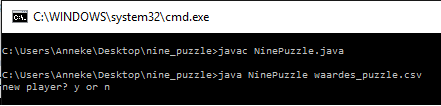
\includegraphics[scale=0.8]{./Prente/prent1.png}
 \caption{New player or not}
 \label{prent1}
\end{figure}
\\
\\Step 4:
\begin{figure}
\centering
 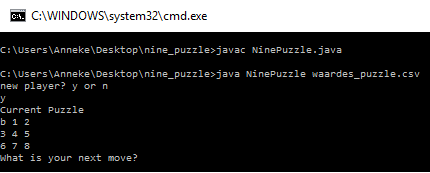
\includegraphics[scale=0.8]{./Prente/prent2.png}
 \caption{The begin puzzle is given to the player}
 \label{prent2}
\end{figure}
\\After Step 3 has been completed the begin puzzle will be given to the player. Figure~\ref{prent2} shows Step 4.
\\
\\Step 5:
\begin{figure}
\centering
 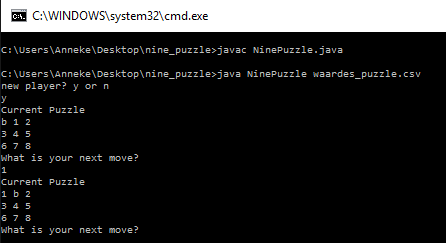
\includegraphics[scale=0.8]{./Prente/prent3.png}
 \caption{After a number has been moved to the empty space}
 \label{prent3}
\end{figure}
\\Enter the number that you want to move to the empty space called "b". Figure~\ref{prent3} shows how the number has been moved to the empty space "b" and gives then the updated puzzle.
\subsection{Functionality}
Stop, save and exit of the program:
\\ Figure~\ref{prent4} shows that the player has type in "0" to save their puzzle to continue at a later stage.
Figure~\ref{prent5} show the message that the program will give to the player is the puzzle have been saved to the .csv file.  After the player has pressed "OK" the program will exit.
\\
\\If the game has been won:
\\Figure~\ref{prent6} will show if the player has won the game by solving the puzzle according to the final puzzle specifying in the .csv file.
\\
\\How to see the goal puzzle that one must obtain from the initial puzzle.
\\Figure~\ref{prent7} shows that the player has entered "99" to see what the goal puzzle must look like.  The program will write "Goal Puzzle" and directly after the goal puzzle have been given the program will give the puzzle that the player must use to obtain the goal puzzle.
\begin{figure*}
  \centering
  \begin{subfigure}{0.5\textwidth}
    \centering
    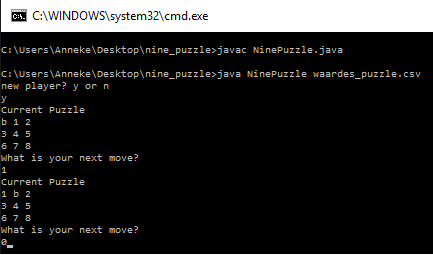
\includegraphics[scale=0.8]{./Prente/prent4.png}
    \caption{If you type in 0}
    \label{prent4}
  \end{subfigure}%
 ~
  \begin{subfigure}{0.5\textwidth}
    \centering
    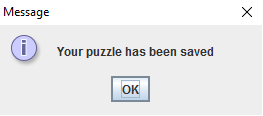
\includegraphics[scale=0.8]{./Prente/prent5.png}
    \caption{Message dialog when the player saves}
    \label{prent5}
  \end{subfigure}
  \caption{\label{2}}
  \end{figure*}
  
\begin{figure}
\centering
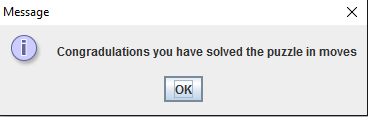
\includegraphics[scale=0.8]{./Prente/prent6.png}
\caption{The congratulation message}
\label{prent6}
\end{figure}

\begin{figure}
\centering
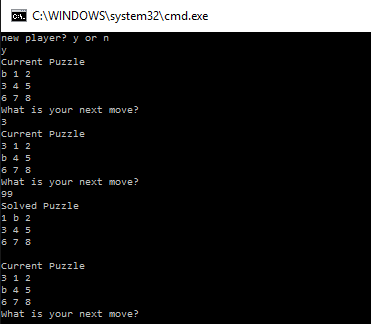
\includegraphics[scale=0.8]{./Prente/prent7.png}
\caption{Goal puzzle is given in the program}
\label{prent7}
\end{figure}

\section{Code}
 \begin{scriptsize}
 \lstinputlisting[language=java, firstline=1, lastline=222]{./NinePuzzle.java}
 \end{scriptsize}

\bibliographystyle{dcu} 
\bibliography{ref}%where the bib file must be read
\end{document}